\documentclass[11pt,a4paper]{article}


\usepackage[T1]{fontenc}
\usepackage[utf8]{inputenc}
\usepackage[spanish,es-nodecimaldot]{babel}
\usepackage{lmodern}
\usepackage{microtype}
\usepackage{amsmath,amssymb,mathtools}
\usepackage{geometry}
\usepackage{enumitem}
\usepackage{booktabs}
\usepackage{tabularx}
\usepackage{xcolor}
\usepackage[hidelinks]{hyperref}

\geometry{margin=2.5cm}
\setlength{\parindent}{0pt}
\setlength{\parskip}{0.45em}
\setlist{itemsep=0.25em,topsep=0.3em}
\renewcommand{\arraystretch}{1.25}
\setcounter{secnumdepth}{0}

\newcommand{\argmax}{\operatorname*{arg\,max}}
\newcommand{\concepto}[1]{%
  \begin{center}
    \fcolorbox{black}{gray!8}{\parbox{0.88\linewidth}{\centering #1}}
  \end{center}%
}

\begin{document}

{\LARGE\bfseries Dynamic Programming\par}
\vspace{0.7em}
{\normalsize\bfseries INTRODUCCIÓN TEÓRICO-PRÁCTICA AL APRENDIZAJE POR REFUERZO\par}
\vspace{0.35em}
\textbf{Profesor:} Matias Bilkis
\hfill
\textbf{Cuatrimestre:} Segundo cuatrimestre 2026

\vspace{0.25em}
\textbf{Integrantes}

\begin{tabularx}{\textwidth}{@{}X@{\hspace{2em}}X@{}}
Agustín Calo \hfill 390/23 & Paz Lavenia \hfill 64/23 \\
Rocco Gasparini \hfill 102/24 & Silvano Picard \hfill 637/24 \\
Maria Delfina Kiss \hfill 72/23 & Ingrid von Foerster \hfill 150/23
\end{tabularx}

\vspace{0.35em}
\hrule

\section{Análisis de Value Iteration}
Usamos el código base de \textit{Value Iteration} que se dio en clase. El entorno modelado es un laberinto representado como una grilla de $n \times n$ con un 20\% de paredes ubicadas al azar y un estado objetivo. El objetivo del experimento fue variar el tamaño de la grilla (desde $n=10$ hasta $n=1000$, en saltos de 100 a partir de $n=1000$) para evaluar cómo escala el algoritmo.


A partir de las ejecuciones, generamos los gráficos de rendimiento (ver Figura \ref{fig:escalabilidad}) y notamos algunos comportamientos:

\begin{figure}[h]
    \centering
    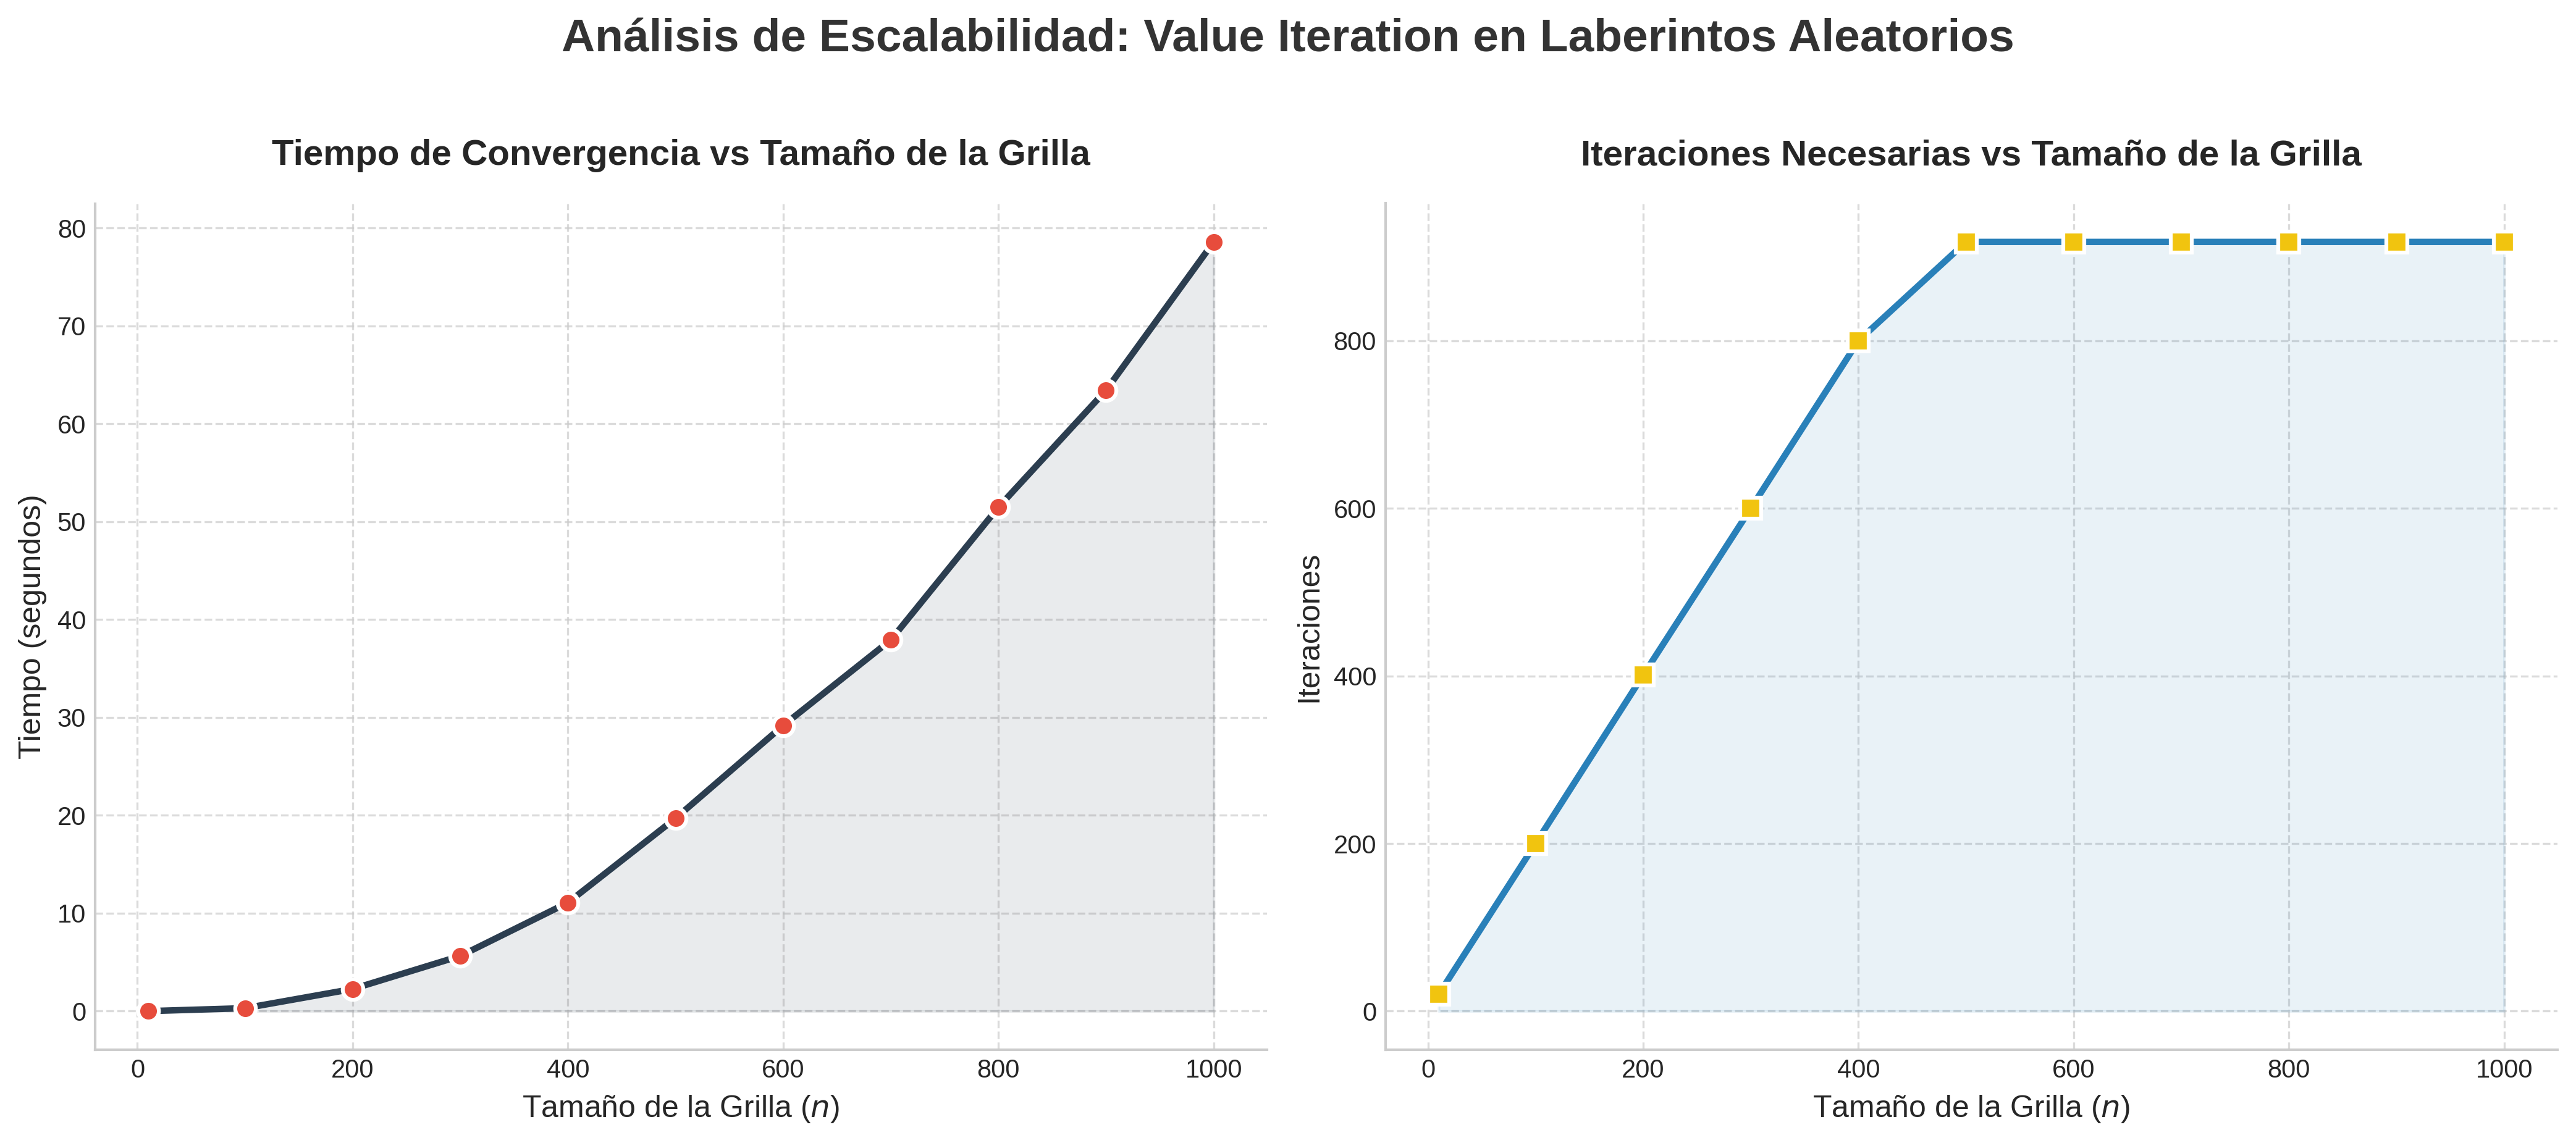
\includegraphics[width=\linewidth]{iteraciones.png}
    \caption{Tiempo de convergencia e iteraciones necesarias en función del tamaño de la grilla.}
    \label{fig:escalabilidad}
\end{figure}

\begin{itemize}
    \item \textbf{Meseta en las iteraciones (gráfico derecho):} Al principio, la cantidad de barridos crece linealmente. Sin embargo, a partir de $n=500$, la curva se estanca por completo en torno a las 900 iteraciones. Esto ocurre por la combinación del factor de descuento ($\gamma = 0.99$) y el umbral de tolerancia ($\theta = 10^{-4}$). Al ser la grilla tan masiva, la recompensa se atenúa tanto con la distancia que, para los estados más alejados, las actualizaciones caen por debajo de $\theta$ y el algoritmo corta antes de que la señal se propague por todo el laberinto.
    
    \item \textbf{Crecimiento polinómico del tiempo (gráfico izquierdo):} La curva temporal se dispara, alcanzando casi los 80 segundos para la grilla más grande. Esto refleja el costo de evaluar matrices donde el total de estados crece cuadráticamente ($n^2$). Para $n=1000$, estamos operando sobre un millón de celdas por iteración.
\end{itemize}

En conclusión, llevar la grilla hasta $n=1000$ ilustra el límite práctico de \textit{Value Iteration}. No solo el tiempo de procesamiento se dispara por el volumen del espacio de estados, sino que la atenuación geométrica de las recompensas impide que el algoritmo resuelva los caminos óptimos completos en distancias extremadamente largas bajo estos hiperparámetros.


\end{document}